
%\vspace{-0.05in}
\section{Markov-chain Monte Carlo Estimators for Score Climbing}
\vspace{-0.05in}
\subsection{Overview of Estimation Strategies}\label{section:overview}
%
\vspace{-0.05in}

\begin{figure*}
    \centering
    \begin{subfigure}[b]{0.25\textwidth}
        \centering
        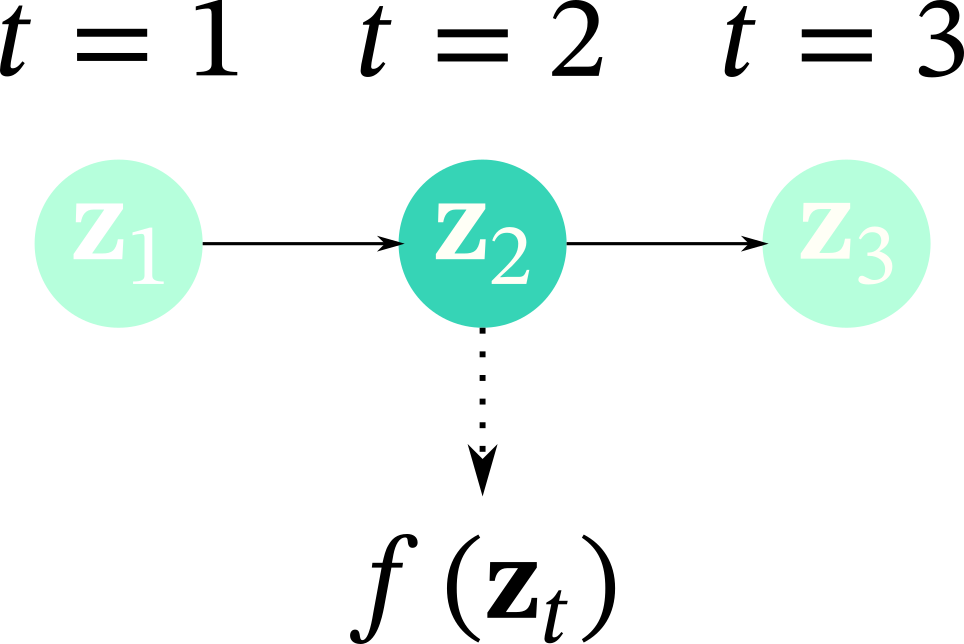
\includegraphics[scale=0.25]{figures/diagram_1.png}
        \caption{Single State Estimator}\label{fig:single}
    \end{subfigure}
    \begin{subfigure}[b]{0.35\textwidth}
        \centering
        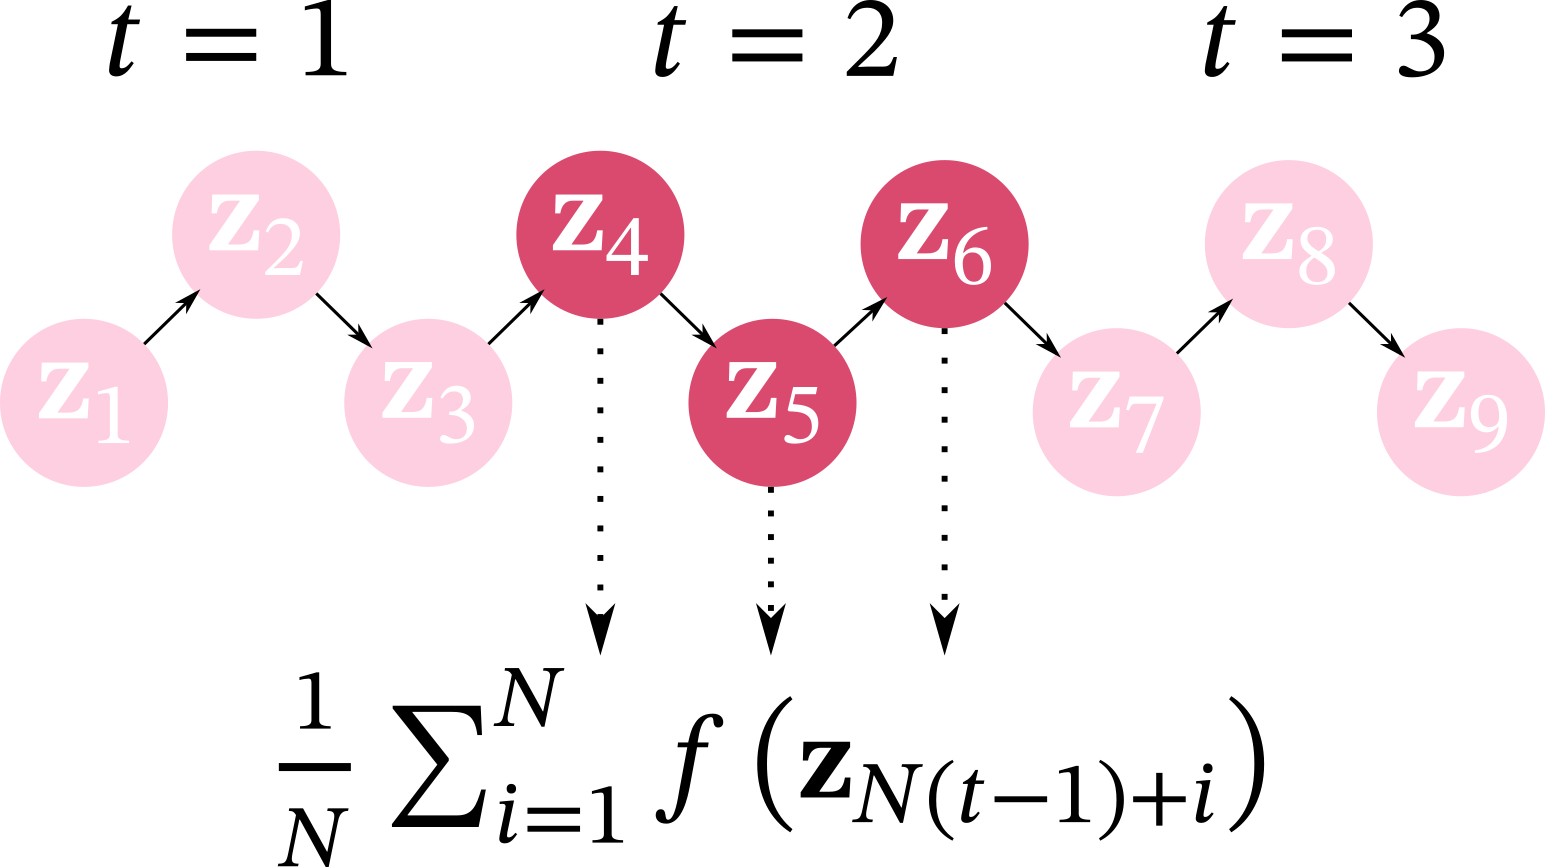
\includegraphics[scale=0.25]{figures/diagram_2.png}
        \caption{Sequential State Estimator}\label{fig:seq}
    \end{subfigure}
    \begin{subfigure}[b]{0.3\textwidth}
        \centering
        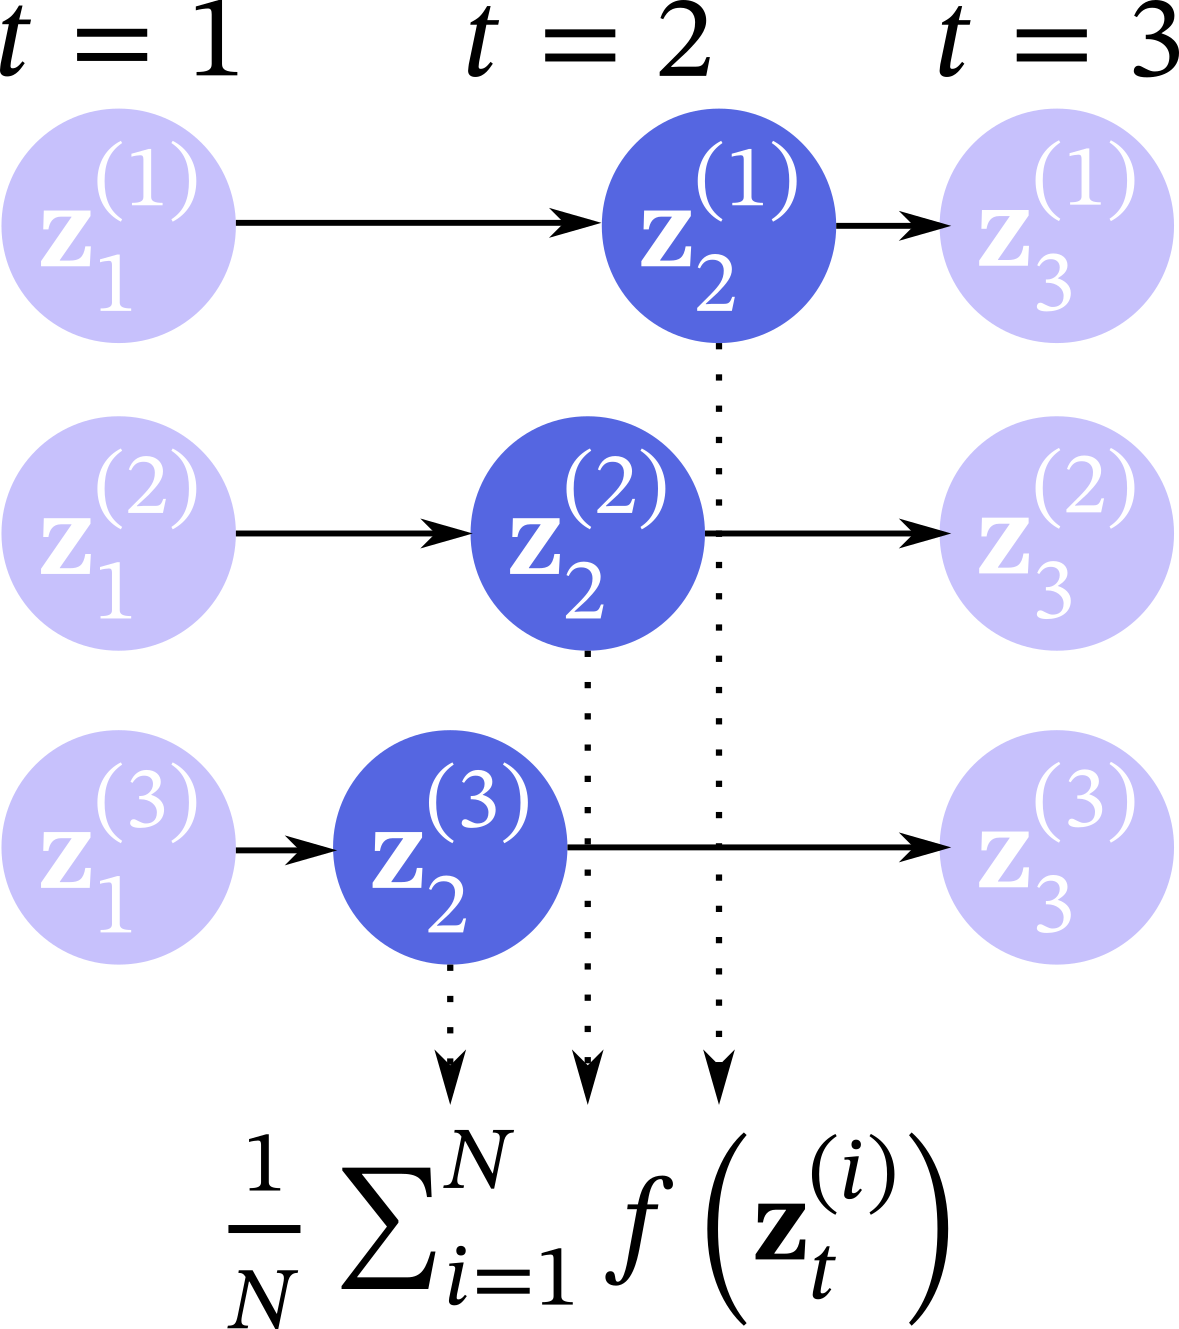
\includegraphics[scale=0.25]{figures/diagram_3.png}
        \caption{Parallel State Estimator (proposed)}\label{fig:par}
    \end{subfigure}
    \caption{Visualization of different ways of combining MCMC with stochastic approximation variational inference.
    The index \(t\) denotes the stochastic approximation iteration.
    The dark circles denote the MCMC samples used for estimating the score gradient at \(t=2\).
    }\label{fig:overview}
\end{figure*}
%

% Second version of table, with booktabs.
%\begin{table}
%\centering
\caption{Computational Costs of MCSA Schemes}\label{table:cost}
\setlength{\tabcolsep}{0.5pt}
  \begin{threeparttable}
\begin{tabular}{lccccc}\toprule
& \multicolumn{3}{c}{\footnotesize Kernel Application} & \multicolumn{2}{c}{\footnotesize Gradient Estimation} \\
\cmidrule(lr){2-4}\cmidrule(lr){5-6}
  & {\footnotesize\(p\left( \vz, \vx \right)\)}
  & {\footnotesize\(q\left(\vz; \vlambda\right)\)}
  & {\footnotesize\(q\left(\vz; \vlambda\right)\)}
  & {\footnotesize\(p\left( \vz, \vx \right)\)}
  & {\footnotesize\( q\left(\vz; \vlambda\right)\)}
  \\
  & {\footnotesize\# Eval.  }
  & {\footnotesize\# Eval.  }
  & {\footnotesize\# Samples}
  & {\footnotesize\# Grad.  }
  & {\footnotesize\# Grad.  }
%
\\\midrule
%
{\footnotesize
ELBO
}
& \(0\)
& \(0\)
& \(N\)
& \(N\)
& \(N\)
\\\arrayrulecolor{black!30}\midrule
%
{\footnotesize
MSC
}
& \(N-1\)
& \(N\)
& \(N-1\)
& \(0\)
& \(1\)\tnote{1}\;\;{\footnotesize or}\;\(N\)\tnote{2}
\\
%
{\footnotesize
JSA
}
& \(N\)
& \(N+1\)
& \(N\)
& \(0\)
& \(N\)
\\
%
{\footnotesize
\textit{pMCSA}
}
& \(N\)
& \(2 \, N\)
& \(N\)
& \(0\)
& \(N\)
\\\bottomrule
\end{tabular}
  \begin{tablenotes}
    \item[*]{\footnotesize We assume that the parameters are cached as much as possible}.
    \item[1]{\footnotesize Vanilla CIS kernel}.
    \item[2]{\footnotesize Rao-Blackwellized CIS kernel}.
  \end{tablenotes}
  \end{threeparttable}
%\end{table}

%

\paragraph{Overview}
Recently,~\citet{NEURIPS2020_b2070693} and~\citet{pmlr-v124-ou20a} proposed two similar but independent methods for performing inclusive variational inference.
Both methods estimate the score gradient by operating a Markov-chain in parallel with the VI optimization sequence.
Also, they both use MCMC kernels that can effectively used the variational approximation \(q_{\vlambda_t}(\vz)\).
Because of this, both methods are much more efficient compared to previous VI approaches~\citep{pmlr-v97-ruiz19a, pmlr-v70-hoffman17a} that used expensive MCMC kernels such as Hamiltonian Monte Carlo.

\vspace{-0.05in}
\paragraph{Single State Estimator}
In Markovian score climbing (MSC), \citeauthor{NEURIPS2020_b2070693} estimate the score gradient by performing an MCMC iteration and update the parameters such that
\vspace{-0.05in}
\begin{align*}
  &\vz_t \sim K_{\vlambda_{t-1}}\left(\vz_{t-1}, \cdot \right) \\
  &g_{\text{single-CIS}}(\vlambda) = s\,(\vz_t; \vlambda)
\end{align*}
where \(K_{\vlambda_{t-1}}\left(\vz_{t-1}, \cdot\right)\) is a MCMC kernel leaving \(p\,(\vz\mid\vx)\) invariant and \(g_{\text{single}}\left(\vlambda\right)\) denotes the score estimator.
For \(K_{\vlambda_{t-1}}\left(\vz_{t-1}, \cdot\right)\), they propose a new type of kernel inspired by particle MCMC~\citep{andrieu_particle_2010, andrieu_uniform_2018}, the conditional importance sampling (CIS) kernel.
Since the estimator uses \textit{a single state} created by the CIS kernel, we call it the single state estimator with the CIS kernel (single-CIS).
The CIS kernel internally uses \(N\) samples from the \(q_{\vlambda_{t-1}}(\vz)\), hence the dependence on \(\vlambda_{t-1}\).
When compared to MCMC kernels that only use a single sample from \(q_{\vlambda_{t-1}}(\vz)\), it is \(N\) times more expensive, but hopefully, statistically superior.

\vspace{-0.05in}
\paragraph{Sequential State Estimator}
On the other hand, at each SGD iteration \(t\),~\citep{pmlr-v124-ou20a} perform \(N\) sequential Markov-chain transitions and use the average of the intermediate states for estimation.
That is, for the index \(i \in \{1, \ldots, N\}\),
\vspace{-0.05in}
\begin{align*}
  &\vz_{T+i} \sim K_{\vlambda_{t-1}}^i\left(\vz_{T}, \cdot \right) \\
  &g_{\text{seq.-IMH}}(\vlambda) = \frac{1}{N} \sum_{i=1}^N s\,(\vz_{T+i}; \vlambda)
\end{align*}
where \(\vz_T\) is the last Markov-chain state of the previous SGD iteration.
\(K^{i}_{\vlambda_{t-1}}(\vz_{T}, \cdot)\) denotes the MCMC kernel sequentially applied \(i\) times.
For the MCMC kernel, they use the classic independent Metropolis-Hastings (IMH,~\citealt[Algorithm 25]{robert_monte_2004}~\citealt{hastings_monte_1970}) algorithm, which uses only a single sample from \(q_{\vlambda_{t-1}}(\vz)\) (notice the dependence on \(\vlambda_{t-1}\) just like the aforementioned CIS kernel).
Therefore, the cost of \(N\) state transitions with IMH is similar to the cost of a single transition with CIS.
Since the estimator uses sequential states, we call it the sequential state esimator with the IMH kernel (seq.-IMH)

%\subsection{The Parallel State Estimator}\label{section:overview}

\paragraph{Overview}
The single and sequential state estimators represent two different ways of using a fixed computational budget.
The former uses a single sample generated in an expensive way, while the latter uses multiple samples generated in a cheap way.
Illustrations of the two schemes are provided in~\cref{fig:single,fig:seq}.

\vspace{-0.05in}
\paragraph{Parallel State Estimator}
In this work, we add a new scheme into the mix: \textit{the parallel state estimator}.
Like the sequential state estimator, we use the cheaper IMH kernel, but instead of applying the MCMC kernel \(N\) times to a single chain, we apply the MCMC kernel a single time to \(N\) \textit{parallel Markov-chains}.
That is, for each Markov-chain \(i \in \{1, \ldots, N\}\),
%
\vspace{-0.05in}
\begin{align*}
  &\vz_{t}^{(i)} \sim K_{\vlambda_{t-1}}\big(\vz_{t-1}^{(i)}, \cdot \big) \\
  &g_{\text{par.-IMH}}(\vlambda) = \frac{1}{N} \sum_{i=1}^N s\,(\vz_{t}^{(i)}; \vlambda)
\end{align*}
%
where \(\vz_{t-1}^{(i)}\) is the state of the \(i\)th chain at the previous SGD step.
Computationally speaking, we are still applying \(K\big(\vz_{t-1}^{(i)}\big)\) \(N\) times in total, so the cost is similar to the sequential state estimator.
However, the Markov-chain are \(N\) times shorter, which, in a traditional MCMC view, might seem to result in worse statistical performance.
An illustration of the parallel state estimator is shown in~\cref{fig:par}, while pseudocodes of the considered schemes are provided in the \textit{supplementary material}.

\vspace{-0.05in}
\paragraph{Computational Cost}
The three scheme using the CIS kernel and the IMH kernel can have different computational cost depending on the parameter \(N\).
The computational costs of each scemes are organized in~\cref{table:cost}.
In the CIS kernel, \(N\) controls the number of internal proposals sampled from \(q_{\vlambda}(\vz)\).
In the sequential and parallel state estimators, the IMH kernel only uses a single sample from \(q_{\vlambda}(\vz)\), but applies the kernel \(N\) times.
When estimating the score, the single state estimator computes \(\nabla_{\vlambda} \log q_{\vlambda}(\vz)\) only once, while for the sequential and parallel state estimators compute it \(N\) times.
However,~\cite{NEURIPS2020_b2070693} also discuss a Rao-Blackwellized version of the CIS kernel, which also computes the gradient \(N\) times.

\subsection{Theoretical Analysis of Bias}\label{section:theory}
\vspace{-0.05in}
\paragraph{Adaptive MCMC and Ergodicity}
For bounded functions, a bound on the bias of MCMC estimators can be easily derived from the convergence rates of MCMC kernels as shown by~\citet[Theorem 4]{jiang_mcmc_2021}.
In the context of MSC, the convergence rate of an MCMC kernel is a subtle subject since the kernel is now \(adaptive\) as it depends on \(\vlambda_t\), which is in turn dependent on all of the past MCMC samples.
This is clearly the type of problem adaptive MCMC algorithms have been concerned with~\citep{andrieu_ergodicity_2006}.
However, our setting crucially differs with adaptive MCMC in that our goal is not to obtain asymptotically unbiased samples.
Instead, we use the MCMC samples acquired during each SGD step, in which \(\vlambda_t\) is fixed.
That is, our MCMC kernel is instantaneously not adaptive, and we are thus we are free to use the ergodicity results of these kernels.
However, we note that, as far as Deoblin's condition holds such that \(w^* = \sup_{\vz, \vlambda} \nicefrac{p\left(\vz\mid\vx\right)}{q_{\vlambda}\left(\vz\right)}  < \infty\) and the SGD stepsize sequence satisfies the diminishing adaptation condition~\citep{10.2307/27595854}, the MCMC kernel will indeed result in asymptotically unbised samples.

\vspace{-0.05in}
\paragraph{Boundedness Assumption}
Since convergence rates are defined with the total-variation distance, our bias results assume that the score function is bounded.
That is, \(\norm{\nabla_{\vlambda} \log q_{\vlambda}(\vz)} < L\) for any \(\vlambda\).
This boundedness assumption is reasonable since theoretical guarentees of SGD often assume Lipschitz-continuity of the gradients, from which boundedness follows as a consequence.
%}

%For the seq.-IMH estimator, the bias is bounded geometrically with the number of states \(N\) and the number of SGD iteration \(t\).
%

\begin{theoremEnd}{propossition}\label{thm:bias_seq}
  Assuming \(w^* = \sup_{\vz} \nicefrac{p\left(\vz\mid\vx\right)}{q_{\vlambda_{t}}\left(\vz\right)} < \infty\; \text{for} \; \forall \vlambda \) and the score function is bounded such that \(\left|\,s(\vz; \vlambda)\,\right| \leq \frac{L}{2}\), the bias of the sequential state estimator with an IMH kernel at iteration \(t\) is bounded as
  {\small
  \[
    \mathrm{Bias}\left[ g_{\mathrm{seq.,\, t}} \right] \leq \frac{L}{N} \, (w^* - 1)
  \]
  }
\end{theoremEnd}
%
\begin{proofEnd}
  We employ a similar proof strategy with the works of~\citet[Theorem 4]{jiang_mcmc_2021}.

  Let us first denote the empirical distribution of the Markov-chain states at iteration \(t\) as
  \begin{align}
    \eta_{\mathrm{seq.},\, t}(\vz) = \frac{1}{N} \sum_{i=1}^N K^{i}(\vz_T, \vz),
  \end{align}
  where \(\vz_{T}\) is the last state of the Markov-chain at the previous SGD iteration.
  Consequently, the estimator can be described as
  \begin{align}
      g_{\mathrm{seq}, t}(\vlambda) = \int s\left(\vz; \vlambda\right) \, \eta_{\mathrm{seq.},\, t}(\vz) \, d\vz.
  \end{align}
  Now,
  \begin{align}
    \DTV{ \eta_{seq.,\, t}(\cdot) }{p\left(\cdot\mid\vx\right)}
    &= \DTV{\frac{1}{N} \sum_{i=1}^N K^{i}(\vz_T, \cdot)}{p\left(\cdot\mid\vx\right)} \\
    &\leq \frac{1}{N} \sum_{i=1}^N  \DTV{K^{i}(\vz_T, \cdot)}{p\left(\cdot\mid\vx\right)} &\text{ (Triangle inequality)}
  \end{align}
 For an IMH kernel with \(w^* < \infty\), the geometric ergodicity of the IMH kernel \citep[Theorem 2.1]{10.2307/2242610} gives the bound
 \begin{align}
   \DTV{K^t(\vz_{0}, \cdot)}{p(\cdot\mid\vx)} \leq {\left(1 - \frac{1}{w^*}\right)}^t.
 \end{align}
 For the SGD step \(t\), \(\vlambda_{t}\) is fixed, temporarily enabling ergodicity to hold.
 Therefore, 
  \begin{align}
    \DTV{ \eta_{\mathrm{seq.},\, t}(\cdot) }{p\left(\cdot\mid\vx\right)}
    &\leq \frac{1}{N} \sum_{i=1}^N {\left( 1 - \frac{1}{w^*} \right)}^i \\
    &=    \frac{1}{N} \sum_{i=1}^N C^i \\
    &=    \frac{1}{N} \left(\frac{ C \left(1 - C^{N}\right)}{1 - C}\right) \\
    &=    \frac{C}{N} \frac{ \left(1 - C^{N}\right) }{1 - C} \\
    &\leq \frac{1}{N} \frac{ C }{1 - C} \\
    &=    \frac{1}{N} \frac{ 1 - \nicefrac{1}{w^*} }{ \nicefrac{1}{w^*} } \\
    &=    \frac{1}{N} \left( w^* - 1 \right)
  \end{align}

  Finally, by the definition of the total-variation distance, 
 \begin{align}
   \mathrm{bias}\left[ g_{\mathrm{seq., t}} \right]
   &\leq \DTV{\eta_{seq.,\, t}(\cdot)}{p(\cdot\mid\vx)} \\
   &\leq \sup_{h : \mathcal{Z} \rightarrow \left[ \text{-}\nicefrac{L}{2}, \nicefrac{L}{2} \right]} \left|\, \Esub{\eta_{\mathrm{seq.},\, t}(\cdot)}{h} - \Esub{p(\cdot\mid\vx)}{h} \,\right| \\
   &= L \, \DTV{ \eta_{\mathrm{seq.},\, t}(\cdot) }{p\left(\cdot\mid\vx\right)}  \\
   &\leq \frac{L}{N} \left( w^* - 1 \right).
 \end{align}
\end{proofEnd}

%%% Local Variables:
%%% TeX-master: "master"
%%% End:

%

\begin{theoremEnd}{theorem}
  Assuming \(w^* = \sup_{\vz} \nicefrac{p\left(\vz\mid\vx\right)}{q_{\vlambda_{\tau}}\left(\vz\right)} < \infty \; \text{for}\;\forall \vlambda \) and that the score function is bounded as \(\left|\, s\left(\vz; \vlambda\right) \,\right| \leq \frac{L}{2}\), the bias of the parallel mode estimator with an IMH kernel at iteration \(t\) is bounded as
  {\small
\[
    \mathrm{Bias}\left[ g_{\mathrm{par.,\, t}} \right] \leq L\,C^t.
\]
  }
  where \(C = 1 - \nicefrac{1}{w^*}\).
\end{theoremEnd}
\begin{proofEnd}
  We denote the empirical distribution of the Markov-chain states at iteration \(t\) as
  \begin{align}
    \eta_{\mathrm{par.},\, t}(\vz) = \frac{1}{N} \sum_{i=1}^N K^{t}\left(\vz_0^{(i)}, \vz\right).
  \end{align}
  and consequently,
  \begin{align}
      g_{\mathrm{par.}, t}(\vlambda) = \int s\left(\vz; \vlambda\right) \, \eta_{\mathrm{par.},\, t}(\vz) \, d\vz.
  \end{align}
  Similarly with~\cref{thm:bias_seq}, 
  \begin{align}
    \DTV{ \eta_{\mathrm{par.},\, t}(\vz) }{p\left(\cdot\mid\vx\right)}
    &= \DTV{\frac{1}{N} \sum_{i=1}^N K^{t}\left(\vz_0^{(i)}, \vz\right)}{p\left(\cdot\mid\vx\right)} \\
    &\leq \frac{1}{N} \sum_{i=1}^N  \DTV{K^t(\vz_0^{(i)}, \cdot)}{p\left(\cdot\mid\vx\right)} &\text{(Triangle inequality)} \\
    &=    \DTV{K^t(\vz_0, \cdot)}{p\left(\cdot\mid\vx\right)} &\text{(Independence)} \\
    &\leq \prod_{\tau=1}^t {\left(1 - \frac{1}{w^*(\vlambda_{\tau})}\right)} \\
    &\leq \prod_{\tau=1}^t {\left(1 - \frac{1}{w^*}\right)} \\
    &\leq C^t
  \end{align}
  where \(w^*(\vlambda_{\tau}) = \sup_{\vz} \nicefrac{p\left(\vz\mid\vx\right)}{q_{\vlambda_{\tau}}\left(\vz\right)} \) and \(C = 1 - \nicefrac{1}{w^*}\).
  And, finally the bias is given as
 \begin{align}
   \mathrm{bias}\left[ g_{\mathrm{par., t}} \right]
   &\leq L \DTV{\eta_{\mathrm{par.},\, t}(\cdot)}{p(\cdot\mid\vx)} \\
   &\leq L \sup_{h : \mathcal{Z} \rightarrow \left[ \text{-}\nicefrac{L}{2}, \nicefrac{L}{2} \right]} \left|\, \Esub{\eta_{\mathrm{par.},\, t}(\cdot)}{h} - \Esub{p(\cdot\mid\vx)}{h} \,\right| \\
   &= L\, \DTV{ \eta_{\mathrm{par.},\, t}(\cdot) }{p\left(\cdot\mid\vx\right)}  \\
   &\leq L \, C^t.
 \end{align}
\end{proofEnd}

%%% Local Variables:
%%% TeX-master: "master"
%%% End:

%
Finally, we analyze the bias of the single-CIS estimator.
Our proof is based on the fact that the CIS kernel is identical to the iterated sampling importance resampling (i-SIR) algorithm by~\citet{andrieu_uniform_2018}.
Especially, we utilize the the convergence rate of the i-SIR kernel.
In addition, we note that the CIS kernel can be reformulated as an accept-reject type kernel that uses Barker's acceptance function~\citep{barker_monte_1965}.
With this perspective, it is identical to the ensemble MCMC sampler independently proposed by~\citet{austad_parallel_2007, neal_mcmc_2011a}.
It can also be found in the review on multiple-try MCMC methods by~\citet[Table 12]{martino_review_2018a}.
%

\begin{theoremEnd}{theorem}
  For a CIS kernel with \(N\) internal proposals,
  assuming \(w^* = \sup_{\vz} \nicefrac{p\left(\vz\mid\vx\right)}{q_{\vlambda}\left(\vz\right)} < \infty\; \text{for} \; \forall \vlambda \), \(N > 2\), and that the score function is bounded such that \(\left|\,s\left(\vz; \vlambda\right)\,\right| \leq \frac{L}{2}\), the bias of the single state estimator at iteration \(t\) is bounded as
  {\small
  \[
    \mathrm{Bias}\left[ g_{\mathrm{cis.,\, t}} \right] \leq L \, C
    \quad\text{where}\quad C = \left(1 - \frac{N}{w^*}\right) < 1.
  \]
  }
\end{theoremEnd}
%
\begin{proofEnd}
  Let us first denote the empirical distribution of the Markov-chain states at iteration \(t\) as
  \begin{align}
    \eta_{\mathrm{cis.},\, t}(\vz) = K\left(\vz_{t-1}, \vz\right),
  \end{align}
  and consequently,
  \begin{align}
      g_{\mathrm{cis}, t}(\vlambda) = \int s\left(\vz; \vlambda\right) \, \eta_{\mathrm{cis.},\, t}(\vz) \, d\vz.
  \end{align}

  The CIS sampler is identical to the iterated sampling importance resampling (i-SIR) algorithm described by~\citet{andrieu_uniform_2018}.
  They showed that the i-SIR kernel achieves a geometric convergence rate such that
  \begin{align}
    \DTV{K^{t}\left(\vz_{t-1},\cdot\right)}{p\left(\cdot\mid\vx\right)}
    &\leq {\left(1 - \frac{N - 1}{2\,w^* + N - 2}\right)}^t.
  \end{align}
  From this, the bound can be shown as
  \begin{align}
    \mathrm{bias}\left[ g_{\mathrm{cis., t}} \right]
   % &\leq \DTV{\eta_{cis.,\, t}(\cdot)}{p(\cdot\mid\vx)} \\
    &\leq \sup_{h : \mathcal{Z} \rightarrow \left[ \text{-}\nicefrac{L}{2}, \nicefrac{L}{2} \right]} \left|\, \Esub{\eta_{\mathrm{cis.},\, t}(\cdot)}{h} - \Esub{p(\cdot\mid\vx)}{h} \,\right| \\
    &= L \, \DTV{ \eta_{\mathrm{cis.},\, t}(\cdot) }{p\left(\cdot\mid\vx\right)}  \\
    &\leq L \, {\left(1 - \frac{N - 1}{2\,w^* + N - 2}\right)} \\
    &\leq L \, {\left(1 - \frac{N}{w^*}\right)} &(\text{Monotonicity})
  \end{align}
  given that \(N > 2\).
\end{proofEnd}

%%% Local Variables:
%%% TeX-master: "master"
%%% End:

%
\begin{figure}[H]
\vspace{-0.05in}
  \centering
  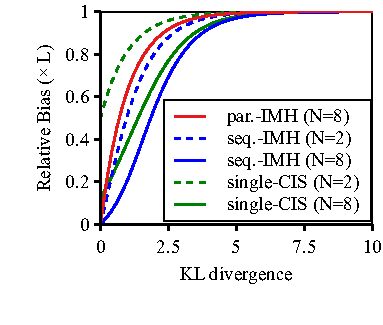
\includegraphics[scale=0.8]{figures/bias_01.pdf}
  \caption{Relative bias of different estimators.
  For simplicity, we take \(w^* = \exp\left( \DKL{p}{q} \right)\).}\label{fig:bias}
\vspace{-0.05in}
\end{figure}
%
\vspace{-0.05in}
\paragraph{Reducing Bias by Increasing \(N\)}
For the seq.-IMH estimator and single-CIS estimator, increasing \(N\) improves the bias decrease rate.
However, it is worth noting that all bias bounds depend on \(w^*\).
By the following proposition, in the initial stages of VI where the KL divergence is large, \(w^*\) is bounded below exponentially.

\begin{theoremEnd}{proposition}
  \(w^* = \sup_{\vz} \nicefrac{p\left(\vz\mid\vx\right)}{q_{\vlambda}\left(\vz\right)} \) is bounded below exponentially by the KL divergence such that
  \[
  \exp\left(\DKL{p\left(\cdot\mid\vx\right)}{ q_{\vlambda}\left(\cdot\right) }\right) \leq w^*.
  \]
\end{theoremEnd}
\begin{proofEnd}
  \begin{align}
    &\DKL{p\left(\cdot\mid\vx\right)}{ q_{\vlambda}\left(\cdot\right) } \\
    &= \int p\left(\vz\mid\vx\right) \log \frac{p\left(\vz\mid\vx\right)}{q_{\vlambda}\left(\vz\right)}\,d\vz \\
    &\leq \int p\left(\vz\mid\vx\right) \log w^* \, d\vz \\
    &= \log w^*
  \end{align}
\end{proofEnd}

Thus, bias reduction is only happens close to convergence of SGD.
In the initial steps, the bias will be large regardless of \(N\) and the method.
To illustrate this point we visualized the bounds in~\cref{fig:bias}.

\subsection{Theoretical Analysis of Variance}
For MCMC estimators, variance often dominate the mean-square error.
Therefore, analyzing the variance is more relevant to practice.

\vspace{-0.05in}
\paragraph{Variance of Single State Estimator}
The variance of the single estimator is given by the law of total variance such as
\begin{align}
  &\V{g_{\text{single}}} \nonumber \\
  &= \E{ \Vsub{K_{\vlambda_{t-1}}\left(\vz_{t-1}, \vz\right)}{ s\left(\vlambda; \vz\right) \mid \vz_{t-1} }} \nonumber \\
  &\quad + \V{ \Esub{K_{\vlambda_{t-1}}\left(\vz_{t-1}, \vz\right)}{ s\left(\vlambda; \vz\right) \mid \vz_{t-1} } }, \\
  \intertext{and assuming stationarity such that \(\vz_{t-1} \sim p\left(\vz \mid \vx\right)\),}
  &= \Esub{p\left(\cdot \mid\vx \right)}{ \Vsub{K_{\vlambda_{t-1}}\left(\vz_{t-1}, \vz\right)}{ s\left(\vlambda; \vz\right) \mid \vz_{t-1} }} \nonumber\\
  &\quad + \Vsub{p\left(\cdot \mid\vx \right)}{ \Esub{K_{\vlambda_{t-1}}\left(\vz_{t-1}, \vz\right)}{ s\left(\vlambda; \vz\right) \mid \vz_{t-1} } } \\
  &= \Vsub{p\left(\cdot\mid\vx \right)}{g_{\text{single}}} \\
  &= \sigma^2
\end{align}
Therefore, ideally, the variance will be equal to the variance of an independent draw from the posterior.
This also suggests that, under stationarity, the variance of the single state estimator will be similar regardless of the MCMC kernel \(K_{\vlambda_{t-1}}\left(\vz_{t-1}, \vz\right)\).

\paragraph{Variance of Parallel State Estimator}
On the other hand, the parallel state estimator can be seen as an average of \textit{i.i.d.} single state estimators.
Therefore, under stationarity, the variance is
\begin{align}
  \V{g_{\text{par.}}} = \frac{\sigma^2}{N}
\end{align}
However, the variance reduction rate does not require stationarity.
Therefore, the parallel state estimator \textit{always} enjoys \(\mathcal{O}\left(\nicefrac{1}{N}\right)\) variance reduction.

\paragraph{Variance of Sequential State Estimator}
Now, assuming stationarity, the variance of the sequential state estimator is given as
\begin{align}
  \V{g_{\text{seq.}}} = \frac{\sigma^2}{N} + \frac{2}{N^2} \sum_{i > j}^N \Esub{p\left(\vz_T \mid \vx \right)}{ \Cov{ \vz_{i}, \vz_{j} \mid \vz_{T} } }\label{eq:var_seq}.
\end{align}
which is similar to the variance of a normal MCMC estimator.
Here, \(T = N\,\left(t - 1\right)\) is the last state of the chain at the previous SGD iteration \(t-1\).
(Detailed derivation is in the \textit{supplementary material}.)
Provided that the covariance term does not exist, the performance will be equal to the parallel state estimator.
However, due to rejections in the MCMC kernel, adjacent states will have some level of correlation.
In the context of VI, the rejection rate will be large when the KL divergence is large as a consequence of~\cref{thm:kl_bound}.
Therefore, in practice, we can expect the performance of the sequential state estimator to be worse than the parallel state estimator.
This is clearly the case as shown in the numerical simulation in~\cref{section:simulation}.

%
%
\begin{theoremEnd}[]{proposition}\label{thm:imh_bound}
  The rejection rate \(r\,(\vz_{t-1})\) of the IMH sampler is bounded below such that
  \[
  %r(\vz_{t-1}) \geq \frac{1}{1 + N\frac{q_{\vlambda}(\vz_{t-1})}{p(\vz_{t-1}\mid\vx)}}.
  r\,(\vz_{t-1}) \geq 1 - \nicefrac{Z}{w\,(\vz_{t-1})} 
  \]
  where \(Z=\int p\,(\vz,\vx) \, d\vz\) is the normalizing constant.
\end{theoremEnd}
\begin{proofEnd}
  The rejection rate \(r(\vz_{t-1})\) is given as
  \begin{align}
    r\,(\vz_{t-1}) = 1 - \int \alpha\left(\vz, \vz_{t-1} \right) \, q_{\vlambda}(\vz) \, d\vz.
  \end{align}
  For an IMH sampler with the Metropolis-Hastings acceptance function and independent proposals, the rejection rate is bounded such that
  \begin{align}
    r\,(\vz_{t-1})
    &= 1 - \int \min\left(\frac{w\,(\vz)}{w\,(\vz_{t-1})}, 1 \right) \, q_{\vlambda}(\vz)\,d\vz \\
    &= 1 - \frac{1}{w\,(\vz_{t-1})} \int \min\Big(w\,(\vz), w\,(\vz_{t-1})\Big) \, q_{\vlambda}(\vz)\,d\vz \\
    &= 1 - \frac{1}{w\,(\vz_{t-1})} \int \min\left(\frac{p\,(\vz,\vx)}{q_{\vlambda}(\vz)}, w\,(\vz_{t-1})\right) \, q_{\vlambda}(\vz)\,d\vz \\
    &=    1 - \frac{1}{w\,(\vz_{t-1})} \int \min\Big(p\,(\vz,\vx), w\,(\vz_{t-1})\,q_{\vlambda}(\vz)\Big) \, d\vz  \\
    &\geq 1 - \frac{1}{w\,(\vz_{t-1})} \int p\,(\vz,\vx) \, d\vz \label{eq:imh_min_comp} \\
    &=    1 - \frac{Z}{w\,(\vz_{t-1})} 
  \end{align}
  The inequality in Equation~\eqref{eq:imh_min_comp} follows from \(\min\big(p\,(\vz,\vx), w\,(\vz_{t-1})\,q_{\vlambda}(\vz)\big) \leq p\,(\vz,\vx) \) for \(\forall \vz \in \mathcal{Z}\).
\end{proofEnd}

%%% Local Variables:
%%% TeX-master: "master"
%%% End:

%

%
\begin{theoremEnd}{proposition}\label{thm:approx_var}
  Assuming \(w\,(\vz_{t-1})\) is large enough to make \(r\,(\vz\mid\vz^{(1:N)})\) independent of \(\vz^{(1:N)}\), the variance can be approximated by
  \begin{align}
    \Vsub{q_{\vlambda}}{ \E{ f \mid \vz_{t-1}, \vz^{(1:N)} } } \approx {\big(1 - r\,(\vz_{t-1})\big)}^2\,\Vsub{q_{\vlambda}}{ f_{\text{IS}} \,\middle\vert\, \vz_{t-1} }.
  \end{align}
\end{theoremEnd}
\begin{proofEnd}
  We evaluate the variance by approximating the rejection probability as an independent constant.
  First,
  \begin{align}
    &\Vsub{q_{\vlambda}}{ \E{ f \mid \vz_{t-1}, \vz^{(1:N)} } }. \\
    \intertext{
      Applying~\eqref{eq:cis_kernel_inter},
    }
    &= \Vsub{q_{\vlambda}}{ \big(1 - r\,(\vz_{t-1}\mid\vz^{(1:N)})\big)\, f_{\mathrm{IS}}
      + r\,(\vz_{t-1}\mid\vz^{(1:N)})\,f(\vz_{t-1}) \;\middle\vert\; \vz_{t-1}} \\
    &\approx \Vsub{q_{\vlambda}}{ \big(1 - r\,(\vz_{t-1})\big)\, f_{\mathrm{IS}}
      + r\,(\vz_{t-1})\,f(\vz_{t-1}) \;\middle\vert\; \vz_{t-1}} \\
    &= \Vsub{q_{\vlambda}}{ \big(1 - r\,(\vz_{t-1})\big)\, f_{\mathrm{IS}} \;\middle\vert\; \vz_{t-1} } \label{eq:approx_var_constant} \\
    &= {\big(1 - r\,(\vz_{t-1})\big)}^2 \, \Vsub{q_{\vlambda}}{ f_{\mathrm{IS}} \;\middle\vert\; \vz_{t-1} }. \label{eq:approx_var_linear} 
  \end{align}
  The equality of~\eqref{eq:approx_var_constant} follows from the fact that \(r\,(\vz_{t-1})\,f(\vz_{t-1})\) is a constant.
\end{proofEnd}

%%% Local Variables:
%%% TeX-master: "master"
%%% End:


%%% Local Variables:
%%% TeX-master: "master"
%%% End:
